\begin{figure*}[!t]
\centering
\begin{subfigure}[t]{0.30\linewidth}
    \centering
    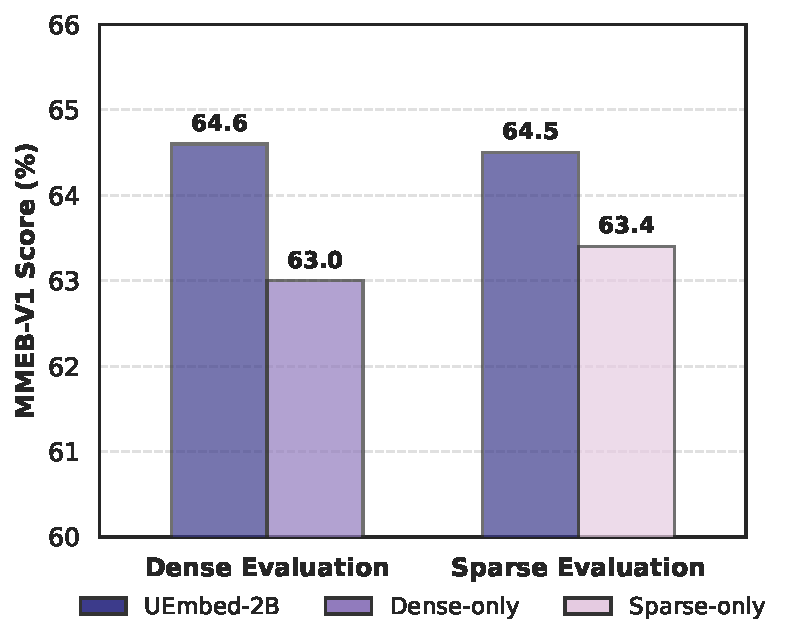
\includegraphics[width=\linewidth]{resources/dense_sparse_mode_bar.pdf}
    \caption{Joint vs.\ single-mode training.}
    \label{fig:dense-sparse-mode-bar}
\end{subfigure}
\hfill
\begin{subfigure}[t]{0.30\linewidth}
    \centering
    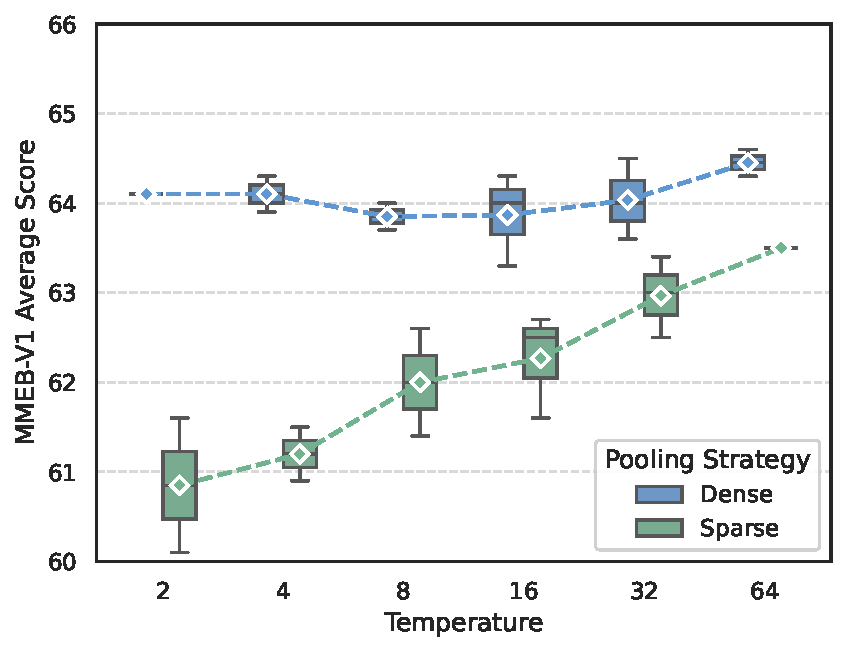
\includegraphics[width=\linewidth]{resources/temp_ablation_boxplot.pdf}
    \caption{Sparse temperature $\tau_s$.}
    \label{fig:temp-ablation-boxplot}
\end{subfigure}
\hfill
\begin{subfigure}[t]{0.30\linewidth}
    \centering
    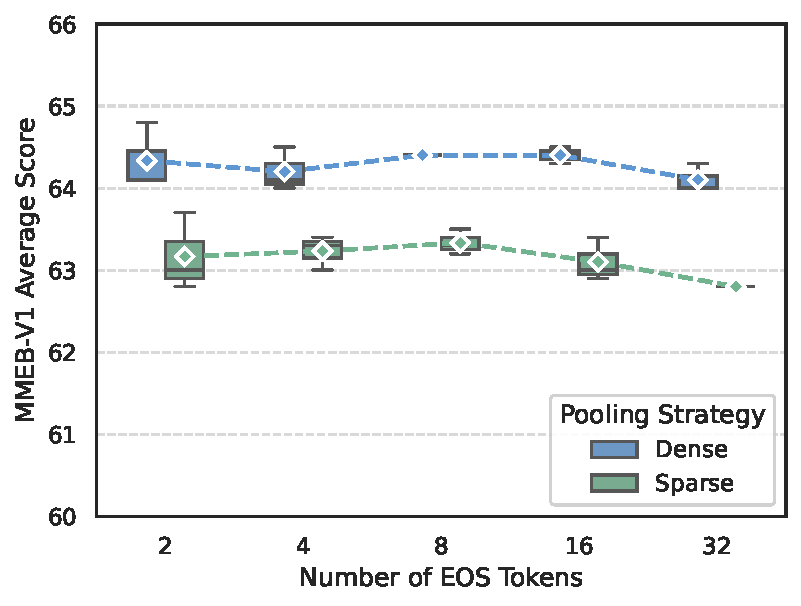
\includegraphics[width=\linewidth]{resources/nes_ablation_boxplot.pdf}
    \caption{Number of special tokens $N$.}
    \label{fig:nes-ablation-boxplot}
\end{subfigure}
\caption{Ablation studies of \ours: (a) joint training matches single-mode specialists; (b)~sweeping the sparse softmax temperature $\tau_s$; and (c)~sweeping the number of appended special tokens $N$.}
\label{fig:ablation-panels}
\end{figure*}
